\documentclass{article}

\usepackage{natbib}
\bibliographystyle{named}
\usepackage[a4paper, total={5.5in, 10in}]{geometry}
\usepackage{graphicx}
\usepackage{hyperref}
\usepackage{listings}
\usepackage{xcolor}
\usepackage{pdfpages}

\author{Bita Mihai-Alexandru, 3B3}
\title{Tema 1}

\begin{document}
\maketitle

\section{Modul de utilizare}
\textbf{Cuvânt inainte: }\emph{executarea acestui program necesită instalat un modul de Python\cite{Python}, iar port-ul 9999 trebuie să fie liber!}\par
Pentru a utiliza acest program se vor efectua, \textbf{în ordine}, următorii pași:
\begin{enumerate}
\item Se deschid 3 terminale în directorul programului.
\item
\begin{enumerate}
\item În primul terminal (\textbf{T1}) se va rula comanda \textcolor{blue}{\lstinline{python server.py}}
\item În al doilea terminal (\textbf{T2}) se va rula comanda \textcolor{blue}{\lstinline{python client_a.py}}
\item În al treilea terminal (\textbf{T3}) se va rula comanda \textcolor{blue}{\lstinline{python client_b.py}}
\end{enumerate}
\item \textbf{T2} va cere, pe parcursul rulării, două input-uri
\begin{enumerate}
\item Primul input specifică modul AES dorit de nodul \textbf{A}: \emph{CBC} sau \emph{CFB}
\item Al doilea input specifică numele fișierului (cu tot cu extensie) care se dorește a fi criptat de nodul \textbf{A}: \emph{nume\_fișier.extensie} sau \emph{"locație\_fișier"/nume\_fișier.extensie}
\end{enumerate}
\item Sfârșitul execuției este indicat de \textbf{T1} printr-un mesaj sugestiv, în timp ce \textbf{T3} va afișa conținutul fișierului cerut la pasul anterior. În cazul unei erori, se inchid toate cele trei terminale și se reiau pașii în aceeași ordine.
\end{enumerate}

\section{Modalitatea de rezolvare}
Rezolvarea temei este alcătuită din patru module: \textcolor{red}{\lstinline{server.py}}, \textcolor{red}{\lstinline{client_a.py}}, \textcolor{red}{\lstinline{client_b.py}} și \textcolor{red}{\lstinline{my_aes.py}}.\par

\subsection{Modulul my\_aes.py}
Acest modul implementează cele două modalități de criptare/decriptare ale algoritmului AES precizate în cerință (\emph{CBC} și \emph{CFB}). Modulul utilizează biblioteca \lstinline{PyCryptodome}\cite{PyCryptodome} pentru a genera string-uri random de 16 bytes și pentru a asigura funcția de criptare/decriptare.
Sunt prezente patru funcții: \textcolor{orange}{\lstinline{cbc_enc()}}, \textcolor{orange}{\lstinline{cbc_dec()}} - pentru criptarea/decriptarea în mod CBC și \textcolor{orange}{\lstinline{cfb_enc()}}, \textcolor{orange}{\lstinline{cfc_dec()}} - pentru criptarea/decriptarea în mod CFB.\par
Toate funcțiile prezentate iau patru parametri:
\begin{itemize}
\item \emph{plaintext}/\emph{ciphertext} - un string de bytes ce urmează a fi criptat sau decriptat
\item \emph{key} - cheia ce va fi folosită la funcția de criptare/decriptare
\item \emph{iv} - vectorul de inițializare
\item \emph{ret\_blocks} - \lstinline{True} dacă se dorește ca funcția să returneze o listă de blocuri sau \lstinline{False} ca funcția să returneze un string de bytes
\end{itemize}
Mai jos sunt prezentate funcțiile. Explicațiile sunt redate în comentarii în limba engleză.\par
\newpage
\begin{center}
\begin{figure}[h!]
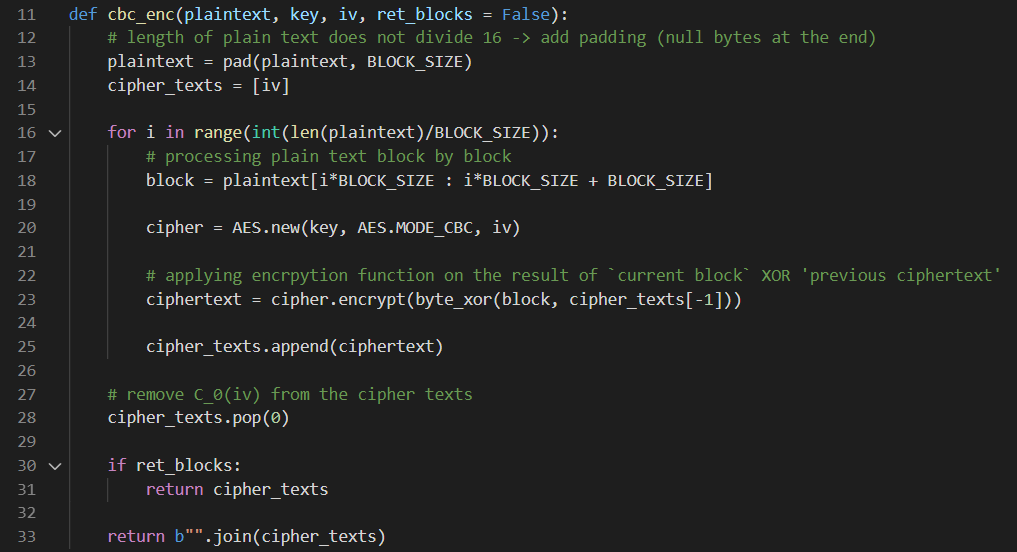
\includegraphics[scale=0.6]{1.jpg}
\caption{funcția de criptare CBC}
\end{figure}
\begin{figure}[h!]
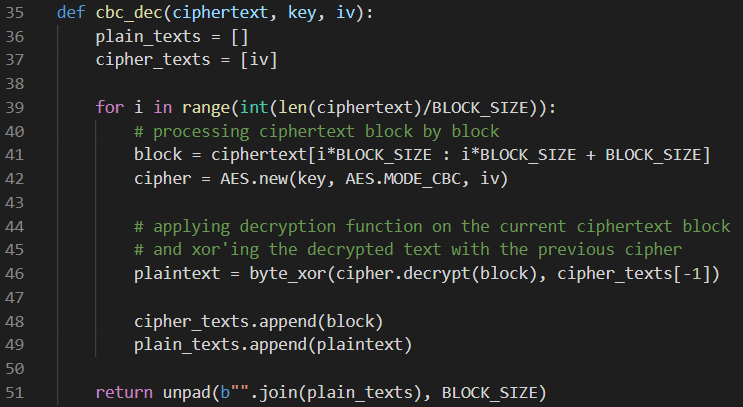
\includegraphics[scale=0.7]{2.jpg}
\caption{funcția de decriptare CBC}
\end{figure}
\begin{figure}[h!]
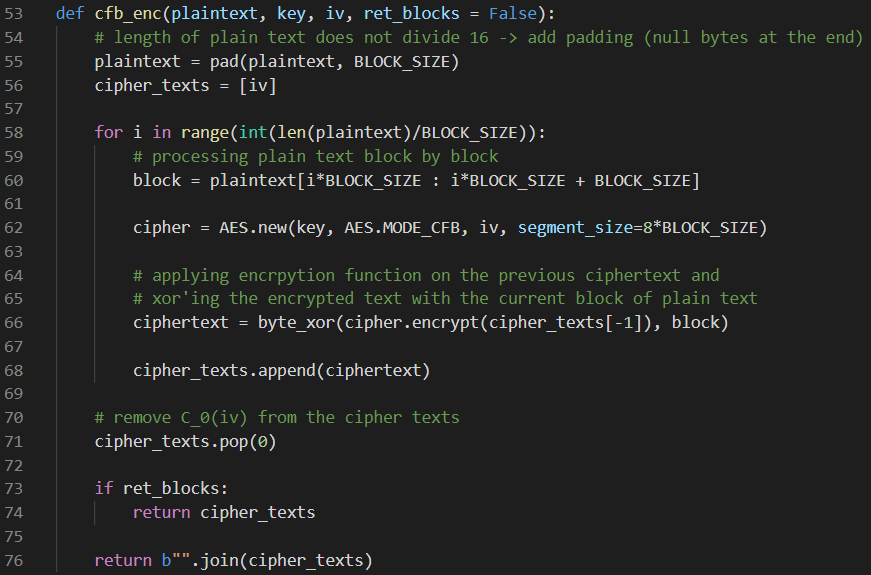
\includegraphics[scale=0.6]{3.jpg}
\caption{funcția de criptare CFB}
\end{figure}
\begin{figure}[h!]
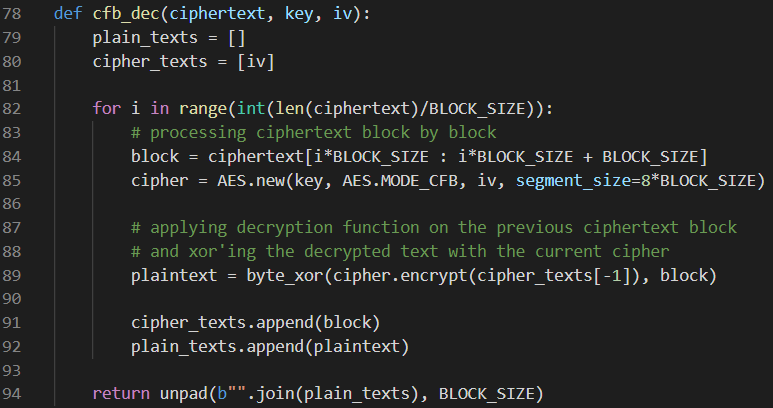
\includegraphics[scale=0.7]{4.jpg}
\caption{funcția de decriptare CFB}
\end{figure}
\end{center}
\newpage

\subsection{Arhitectura server-client}
Modulul \textcolor{red}{\lstinline{server.py}} creează un server TCP ce servește maximum doi clienți (nodurile \textbf{A} și \textbf{B}) folosind \emph{thread-uri}. Astfel, putând partaja memoria, se cunoaște etapa la care se află rezolvarea problemei în orice instanță de timp.\par
Fiecare \emph{thread} se ocupă de comunicarea cu nodul care i-a fost atribuit. Un nod se conectează la server prin modulul \textcolor{red}{\lstinline{client_a.py}} sau \textcolor{red}{\lstinline{client_b.py}}. Primul care se va conecta va fi nodul \textbf{A}, așadar o va face prin \textcolor{red}{\lstinline{client_a.py}}, iar \textbf{B} prin \textcolor{red}{\lstinline{client_b.py}}.\par
Conexiunile se închid automat atunci când procedeul s-a sfârșit cu succes sau manual atunci când a fost întâmpinată o eroare. Toate etapele sunt jurnalizate pe ecranul fiecărui terminal.\par

\begin{center}
\begin{figure}[h!]
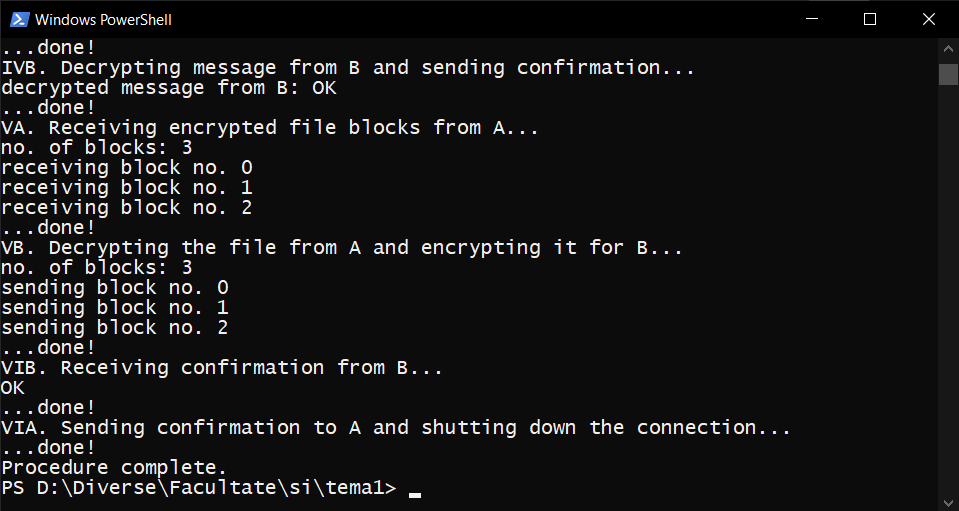
\includegraphics[scale=0.7]{5.jpg}
\caption{rezultatul unei proceduri complete la ecranul lui \textbf{T1}}
\end{figure}
\begin{figure}[h!]
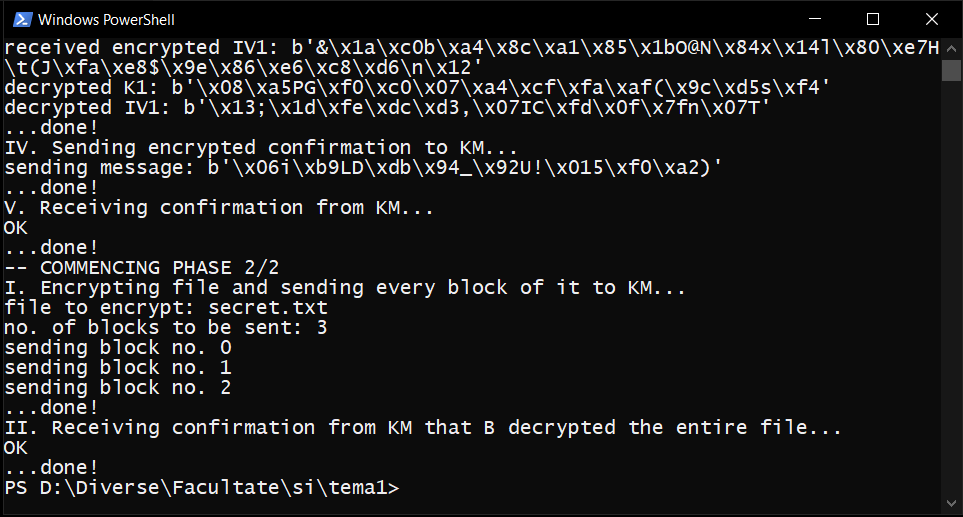
\includegraphics[scale=0.7]{6.jpg}
\caption{rezultatul unei proceduri complete la ecranul lui \textbf{T2}}
\end{figure}
\newpage
\begin{figure}[h!]
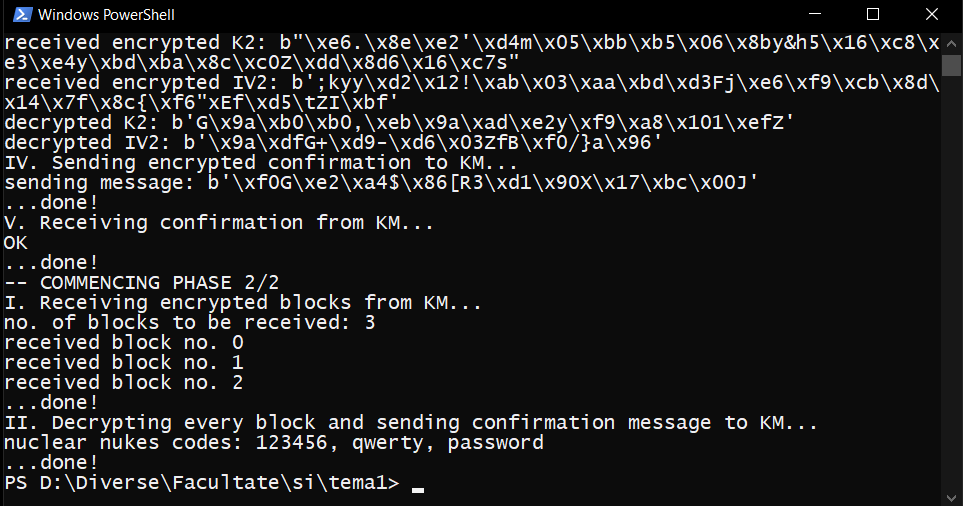
\includegraphics[scale=0.7]{7.jpg}
\caption{rezultatul unei proceduri complete la ecranul lui \textbf{T3}}
\end{figure}
\end{center}


\begin{thebibliography}{9}
\bibitem{Python}
Python
\url{https://www.python.org/}
\bibitem{PyCryptodome}
PyCryptodome
\url{https://pycryptodome.readthedocs.io/}
\end{thebibliography}  

\end{document}
